
\pagebreak

\section*{Introduction}
\addcontentsline{toc}{section}{Introduction}

Le transport aérien de fret s'est développé à partir de 1911 lors d'un
premier vol dont l'objet était de livrer 15 kg de courrier entre deux villes asiatiques distantes de 10 km sur un biplan Sommer. 

%Depuis, le traffic a "légèrement" augmenté pour atteindre en 2014, 51 millions de tonnes pour une valeur de US\$6.8 trillions \cite{RePEc:eee:jaitra:v:61:y:2017:i:c:p:34-40}.

Aujourd'hui, le fret aérien, au même titre que le transport de passagers, continue de jouer un rôle majeur dans l'économie, le développement international et plus fondamentalement dans notre manière d'appréhender le monde au même titre que son pendant virtuel, l'Internet. 


%La présente étude vise à effectuer une analyse de marché suivant le modèle des 5 forces de Porter.
%Le modèle de Porter consiste à effectuer l'analyse de marché suivant 5 domaines :
%la concurrence dans le secteur, deux menaces : les nouveaux entrants et les substituts et deux déterminants : pouvoir de marché des clients et fournisseurs.
%
%\begin{figure}[H]
%	\begin{center}
%		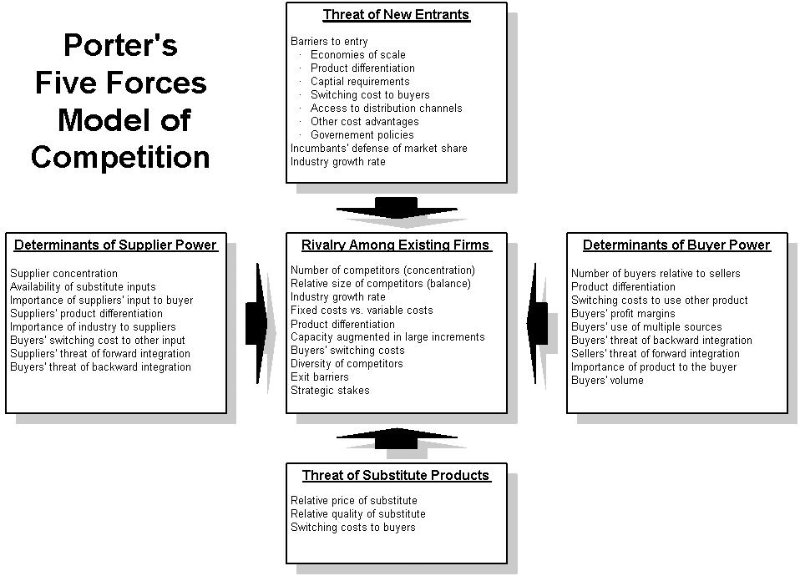
\includegraphics[scale=0.48]{images/porter/porter_1}
%		\caption{Modèle de Porter}
%		\label{inclusion}
%	\end{center}
%\end{figure}
%
%
%Suivront une étude du rôle de l'Air Traffic Management (ATM) dans la stratégie des acteurs du secteur et de son évolution future au regard de ces stratégies des acteurs du secteur. 
%   



